Having constructed an index on a document collection, queries need to 
be matched to documents and a list of answers returned. We need a ranking algorithm based on good mathematical retrieval models to 
return relevant documents at top of the ordered list, leading to high effectiveness. 
Three well-known retrieval models are~\citep{croft2010search}: (1) vector space models (e.g., term frequency and inverse document frequency (TF-IDF)), (2) probabilistic models (e.g., BM25\footnote{BM stands for Best Match, and 25 is just a numbering scheme used by~\cite{robertson1994some} to keep track of weighting variants.}), and (3) Language Models~(LM). 

\paragraph{The Vector Space Model}
\ \\
In a vector space model, documents and queries are represented by vectors of term weights, and the collection is represented by a matrix of term weights as follows: 
\begin{displaymath} 
D_{i}=[d_{i1}, d_{i2}, d_{i3}, \ldots , d_{im}],
\end{displaymath}
\begin{displaymath} 
Q=[q_{1}, q_{2}, q_{3}, \ldots , q_{m}],
\end{displaymath}
\begin{displaymath} 
C=
%\begin{matrix} D_{1} \\ D_{2} \\ D_{3} \\ \vdots\\ D_{N} \\\end{matrix}
\begin{bmatrix}
        d_{11} & d_{12} & d_{13} & \cdots & d_{1m}\\
        d_{21} & d_{22} & d_{23} & \cdots & d_{2m}\\
        d_{31} & d_{32} & d_{33} & \cdots & d_{3m}\\
        \vdots\\
        d_{N1} & d_{N2} & d_{N3} & \cdots & d_{Nm}
     \end{bmatrix},
\end{displaymath}
%\capstartfalse
%\begin{figure}[htpb]
%   \centering
%   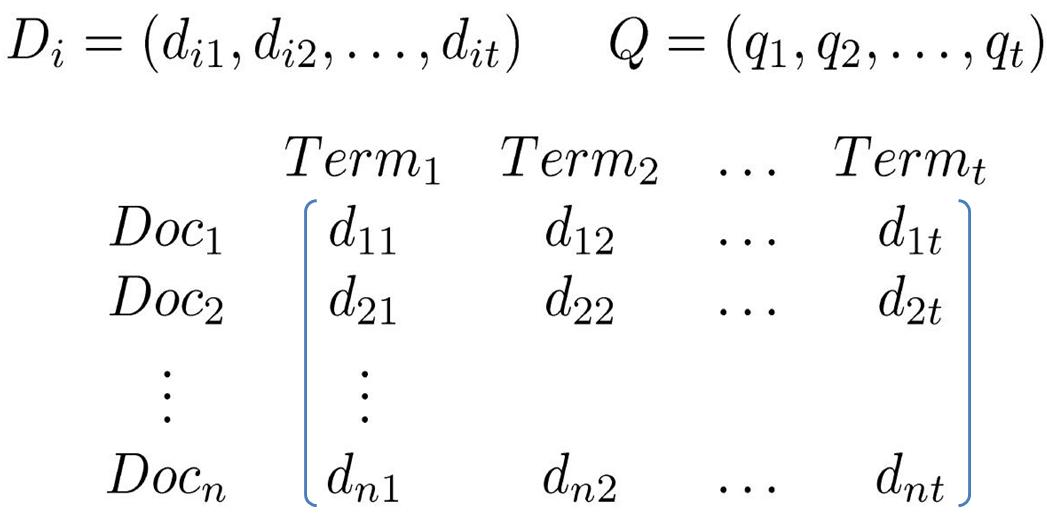
\includegraphics[width=.45\textwidth,height=35mm]{figs/vsm-matrix.jpg}
%\end{figure}
%\capstarttrue
%\FloatBarrier 
\noindent
where $ D_{i} $ is a document in the collection $ C $, $ d_{ik} $ is a weight for each term $ t_{k} $ in the document $ D_{i} $, and $ q_{k} $\footnote{We ignore indices to simplify the equations in this thesis.} represents a term in the query $ Q $. The collection is represented by the matrix $C_{Nm}$, where $N$ is the number of documents in the collection and $m$ is the number of all vocabularies. If a term does not appear in a document or a query, the weight for that particular term will be zero. 

The TF-IDF weighting function multiplies the occurrence of each term in the document ($ c(t_{k},Di)$)
by the inverse document frequency ($ idf $) measure. $ idf $ measures the importance of a term in the collection: 
\begin{equation}
idf(t_{k})=\log\frac{N+1}{df(t_{k})},
\label{eq:idf}
\end{equation}
where $ df(t_{k}) $ is the number of documents in the collection, which contain at least one occurrence of the term $ t_{k} $, and $ N $ is the number of documents in the collection. 

Given a query $Q$, documents are ranked based on the overlap score measure. The TF-IDF score of a document $D$ is the sum, over all query terms, of the TF-IDF weight of each query term $q$ in $D$. After pivoted normalisation, the TF-IDF score for each document is calculated as follows~\citep{bache2010improving}:
\begin{equation}
TFIDF(Q,D)=\sum\limits_{q \in Q\cap D}\frac{c(q,D)\times idf(q)}{(1-b)+b.\frac{|D|}{avdl}},
\label{eq:tfidf}
\end{equation}
where $ |D| $ is the size of the document (i.e, the number of words) and $ avdl $ is the average document length, $ c(q,D)$ is the number of occurrence of each query term in the document $D$, and $idf(q)$ is the importance of each query term in the collection. TF-IDF model scores a document higher if more query terms are present or these terms are rarer in the collection. The parameter $ b $ is set to 0.75 to be the same as the BM25 model as will be described below.
\paragraph{Probabilistic Models}
\ \\
BM25 is a popular and effective ranking algorithm, which extends the scoring function for the binary independence model~\citep{manning2008introduction} to include document and query term weights. Each document is scored based on the BM25 weighting scheme --- often called the Okapi weighting --- as follows:
\begin{equation}
BM25(Q,D)=\sum\limits_{q \in Q\cap D}\Bigg(\log\frac{N+1}{df(q)}\Bigg)\Bigg(\frac{(k_{1}+1)c(q,D)}{k_{1}((1-b)+b.\frac{|D|}{avdl})+c(q,D)}\Bigg).
\label{eq:idfbm25}
\end{equation}
The variable $ k_{1} $ is a positive tuning parameter that calibrates the document term frequency scaling. The setting of $ k_{1}=0 $ corresponds to a binary model (i.e., no term frequency), and setting a large value for $ k_{1} $ corresponds to using raw term
frequency. The parameter $ b $ is also used for tuning ($ 0 \leq b \leq 1 $) which determines the scaling by document length: $ b = 1 $ corresponds to fully scaling the term weight by the document length, while $ b = 0 $ corresponds to no length normalisation. 

If the query is long, then we might also use similar weighting for query terms. This is appropriate if the queries are paragraph long information needs, but unnecessary for short queries.
\begin{equation}
BM25(Q,D)=\sum\limits_{q \in Q\cap D}\log\Bigg(\frac{N+1}{df(q)}\Bigg)\Bigg(\frac{(k_{1}+1)c(q,D)}{k_{1}((1-b)+b\frac{|D|}{avdl})+c(q,D)}\Bigg)\Bigg(\frac{(k_{3}+1)c(q,Q)}{k_{3}+c(q,Q)}\Bigg),
\label{eq:idfbm25}
\end{equation}
where $ c(q,Q) $ is the frequency of term $ q $ in the query $ Q $, and $ k_{3} $ being another positive tuning parameter that this time calibrates term frequency scaling of the query. In the equation presented, there is no length normalisation of
queries because retrieval is being done with respect to a single fixed query. The tuning parameters of these equations should ideally be set to optimise performance on a development test collection. That is, we can search for values of these parameters that maximise performance on a separate development test collection (either manually or with optimisation methods such as grid search or something more advanced), and then use these parameters on the actual test collection. In the absence of such optimisation, experiments have shown reasonable values are to set $ k_{1} $ and $ k_{2} $ to a value between 1.2 and 2, and b = 0.75~\citep{manning2008introduction}.

\paragraph{Language Models with Terms Smoothing}
\ \\
The basic idea behind the \textit{Language Modelling} approach is to estimate a language model for each document, and rank documents by the likelihood of the query according to the estimated language model. Here terms are assumed to occur independently, and the probability is the product of the individual query terms given the document model $ M_{D} $ of document $ D $:
\begin{equation}
\label{eq:multinomial}
 P(Q|M_{D}) = \prod\limits_{q\in Q} P(q|M_{D}) 
\end{equation}

\begin{equation}
\label{eq:multinomial}
 P(q|M_{D}) = \frac{c(q,D)}{|D|}
\end{equation}

The overall similarity score for the query and the document could be zero if some of query terms do not occur in the document. However, it is not sensible to rule out a document just because a single query term is missing. For dealing with this, language models make use of smoothing to balance the probability mass between occurrences of terms in documents, and terms not found in the documents.
\\\\
\textit{Jelinek-Mercer smoothing.} Jelinek-Mercer smoothing language model~\citep{zhai2004study} combines the relative frequency of a query term $ q\in Q $ in the document $ D $ with the relative frequency of the term in the collection (\textit{C}) as a whole. With this approach, the maximum likelihood estimate is moved uniformly toward the collection model probability $ P(q|C) $:
\begin{equation}
P(q|M_{D}) = (1-\lambda)\frac{c(q,D)}{|D|}+\lambda P(q|C) 
\label{eq:jmsmoothing}
\end{equation} 
$ c(q,D) $ represents the frequency of term $ q $ in document $ D $. The optimal value of $ \lambda $ depends on both the collection and the query. It is normally suggested as ($ \lambda = 0.1$) for title queries and ($ \lambda = 0.7$) for long queries.
\\\\
\textit{Dirichlet (Bayesian) smoothing (DirS).} As long documents allow us to estimate the language model more accurately, Dirichlet smoothing ~\citep{zhai2004study} smooths them less. If we use the multinomial distribution to represent a language model, the conjugate prior of this distribution is the Dirichlet distribution. This gives:
\begin{equation}
\label{eq:bayessmoothing}
 P(q|M_{D}) = \frac{c(q,D) + \mu P(q|C)}{|D| + \mu}
\end{equation} 

The formula assign negative score to documents that contain the term, but with fewer occurrence than predicted by the collection language model. As $ \mu $ gets smaller, the contribution from the collection model also becomes smaller, and more emphasis is given to the relative term weighting. Precision is more sensitive to $ \mu $ for long queries, especially when $ \mu $ is small. When $ \mu $ is sufficiently large, long queries perform better than short queries. The optimal value of $ \mu $ varies from collection to collection, though in most cases, it is around 2000. The performance is more sensitive to smoothing for verbose queries. Long queries also require more aggressive smoothing to achieve optimal performance. 